\documentclass[../sections/capitulo_1.tex]{subfiles}
\usetikzlibrary{shapes,backgrounds}
\begin{document}

\begin{center}
    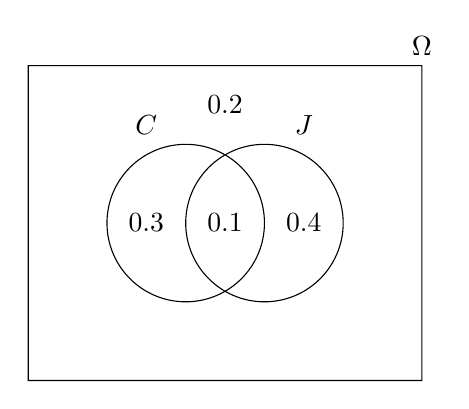
\begin{tikzpicture}[fill=gray]
        % left hand
        \scope
        \clip (-2,-2) rectangle (2,2)
              (1,0) circle (1);
        % \fill (0,0) circle (1);
        \endscope
        % right hand
        \scope
        \clip (-2,-2) rectangle (2,2)
              (0,0) circle (1);
        % \fill (1,0) circle (1);
        \endscope
        % outline
        \draw (0.5,0) node {$0.1$} (0.5,1.5) node {$0.2$}
              (0,0) circle (1) (-0.5,1)  node [text=black,above] {$C$} (-0.5,0) node {$0.3$}
              (1,0) circle (1) (1.5,1)  node [text=black,above] {$J$} (1.5,0) node {$0.4$}
              (-2,-2) rectangle (3,2) node [text=black,above] {$\Omega$} ;
    \end{tikzpicture}
\end{center}

\end{document}